\chapter{Épidémiologie comparée du chikungunya et du Zika} 
\chaptermark{}


Les maladies transmises par les moustiques du genre {\em Aedes} ont pris une importance grandissante depuis le début du XXI\textsuperscript{ème} siècle, en particulier avec les émergences explosives du chikungunya et du Zika, et la résurgence de la dengue et de la fièvre jaune.
Les trajectoires récentes du chikungunya et du Zika présentent de nombreuses similitudes.
Cela suggère que le mode de transmission commun à ces deux maladies joue un rôle fondamental dans leur propagation locale et internationale.
Toutefois, si la survenue d'une épidémie tient largement à la présence conjointe d'un virus adapté, d'hôtes susceptibles et de vecteurs compétents, de nombreux facteurs sont impliqués dans les dynamiques locales de transmission des maladies vectorielles.
Ces facteurs intriqués peuvent être en lien avec des caractéristiques du virus (comme la probabilité de transmission par piqûre ou les durées d'incubation chez l'hôte et le vecteur), des hôtes (comme la densité, la répartition spatiale ou la structure socio-économique de la population touchée), et des vecteurs (comme le types d'espèces présentes et leur compétences vectorielles respectives ou l'abondance des moustiques en relation avec les conditions environnementales locales).

Dans ce contexte, il est primordial d'améliorer les connaissances scientifiques générales sur les dynamiques épidémiques des maladies transmises par les moustiques du genre {\em Aedes}. 
Mieux comprendre l'importance relative de ces facteurs, et distinguer ce qui relève de particularités locales et de principes plus généraux pourrait permettre d'améliorer la préparation des systèmes de surveillance, de prévention et de soin en cas de nouvelle émergence.
L'analyse comparée d'épidémies successives de maladies partageant le même mode de transmission, et survenant au sein des mêmes populations dans les mêmes zones permet de répondre à ces questions.
Avec cet objectif, nous présentons dans ce chapitre un travail d'{\em épidémiologie comparée} des dynamiques épidémiques du chikungunya et du Zika dans neuf territoires de Polynésie française et des Antilles françaises.

\section[Présentation de l'étude]{Présentation de l'étude}

\subsection{Données utilisées et justifications}

Dans ce travail, nous avons choisi de nous concentrer sur les données d'incidence hebdomadaire concernant les épidémies successives de chikungunya et de Zika s'étant produites à un ou deux ans d'intervalle dans six îles ou petits archipels de Polynésie française et trois îles des Antilles françaises entre 2013 et 2016 (Fig. \ref{fig:profiles}).
\begin{figure}[t]
	\centering
	\includegraphics[width=15.5cm]{Figures/Fig1_revised2.pdf}
	\caption{Profils d'incidence des épidémies de chikungunya (en rouge) et de Zika (en bleu) dans six îles de Polynésie française et trois îles des Antilles françaises entre 2013 et 2016 (sources : {\em Centre d'Hygiène et de Salubrité Publique de Polynésie française} et {\em CIRE Antille-Guyane}).}
	\label{fig:profiles}
\end{figure}
Plusieurs raisons justifient ce choix.
D'abord, ces épidémies partagent de nombreuses caractéristiques.
Il s'agit de maladies émergentes, circulant pour la première fois dans les zones étudiées, ce qui permet de faire l'hypothèse que les populations touchées étaient dans les deux cas entièrement susceptibles au début de la période épidémique
Ces épidémies sont survenues successivement en un court laps de temps dans les mêmes territoires, ce qui permet de faire l'hypothèse de la stabilité d'une épidémie à l'autre de nombreuses caractéristiques non-observées liées à ces territoires, relevant de la population, des vecteurs et de l'environnement.
On peut aussi faire l'hypothèse de la stabilité des systèmes de surveillance, d'autant plus que ces deux maladies causent le même type de symptomatologie.
Le chikungunya et le Zika partagent surtout le même mode de transmission, si on néglige la transmission sexuelle du Zika qui est considérée comme faible \cite{althaus_how_2016}.
Malgré le fait que des données sur les cas rapportés de dengue soient disponibles dans ces zones, nous n'avons pas inclus cette maladie du fait de sa circulation ancienne, modifiant la susceptibilité des populations et donc les dynamiques épidémiques.
De plus, la complexité immunologique de la dengue, avec l'interaction entre ses différents sérotypes, complexifierait l'analyse.
Il faut aussi noter que malgré la large propagation de ces maladies dans les zones tropicales d'une grande partie du monde à partir de 2005, peu d'épidémies ont fait l'objet d'une surveillance par un système établi et fiable.
Enfin, le fait que ces épidémies surviennent dans des îles de taille relativement faible facilite l'analyse, car cela rend plus acceptable l'hypothèse que les données d'incidence obtenues concernent une seule épidémie circonscrite à une population donnée.
Au contraire, lorsque des épidémies sont observées dans un territoire plus large, la question de l'échelle d'analyse la plus adaptée est toujours délicate.

\subsection{Objectifs et stratégie d'analyse}
\label{sec:presenttsir}

Nous proposons une analyse comparée d'épidémies de chikungunya et de Zika dans différents territoires ayant pour objectifs de distinguer l'influence exercée sur les dynamiques épidémiques
\begin{enumerate}
\item[(1)] par les caractéristiques propres à chaque virus, généralisables à d'autres situations ;
\item[(2)] par des conditions météorologiques variant au cours et entre les épidémies ;
\item[(3)] et par des facteurs dépendants des propriétés du contexte local où l'épidémie se produit, et qui peuvent être considérées comme stables sur la durée qui sépare la survenue des deux épidémies.
\end{enumerate}
L'analyse repose sur l'ajustement d'un modèle conjoint {\em hiérarchique} à l'ensemble des données d'incidence disponibles pour les dix-huit épidémies retenues.
On considère deux éléments principaux.

Premièrement, la reconstruction mécaniste de la distribution de l'intervalle de génération pour les deux maladies, prenant en compte l'influence de la température locale sur l'activité des vecteurs (plus spécifiquement l'association entre d'une part la température et d'autre part la durée de la période d'incubation extrinsèque et la durée d'un cycle gonotrophique, cf. annexe A).

Deuxièmement, le développement d'une extension au modèle TSIR.
Ce modèle, déjà présenté au paragraphe \ref{sec:tsir}, envisage la génération du nombre cas secondaires observés par semaine $O_t$ lors d'une épidémie selon trois paramètres : un paramètre de taux de signalement $\rho$, un paramètre de transmission $\beta$ et un paramètre de surdispersion $\phi$.
Ainsi, pour rappel, \textit{une} épidémie émergente dans \textit{une} population donnée est décrite par :
\begin{equation} 
O_t|\rho,\beta,\phi \sim \text{Binom-Neg}\left(S_t\frac{\beta}{N} \sum_{u=1}^{t-1} w(u,T_t) O_{t-u}, \phi \right)
\end{equation}
où la fonction de densité discrétisée de probabilité de l'intervalle de génération $w(u,T_t)$ est maintenant dépendante de la température locale $T_t$.
Ce modèle a été étendu afin de correspondre aux données utilisées (dix-huit épidémies et non une seule) et aux objectifs de l'étude.
Considérons maintenant l'épidémie du virus $j$ dans l'île $i$.
Le taux de signalement $\rho_{ij}$ est maintenant modélisé par :
\begin{equation}
\ln \frac{\rho_{ij}}{1-\rho_{ij}}=   r_i   + V_{j}  \ln \omega 
\end{equation}
où $r_i \sim N(\mu_\rho, \sigma_\rho^2)$ permet d'introduire un effet aléatoire par île, où $V_j$ est égal à $1$ pour ZIKV et à $0$ pour CHIKV, et où $\omega$ est l'odds-ratio entre le taux de signalement d'un cas de ZIKV et le taux de signalement d'un cas de CHIKV durant l'épidémie. 
De façon similaire, le paramètre de transmission $\beta_{ijt}$ suit :
\begin{equation}
\label{eqn:beta}
\ln \beta_{ijt} = b_{i} + V_j \ln\beta_D   + \sum_{l=0}^{8} T_{t-l} \ln\beta_{T,l}  + \sum_{l=0}^{8} P_{t-l} \ln\beta_{P,l} 
\end{equation}
où $b_{i} \sim \mathcal{N}(\mu_{B}, \sigma_{B}^2)$ est l'effet aléatoire par île, $\beta_D$ est le ratio entre le paramètre de transmission de ZIKV et le taux de transmission de CHIKV, et les deux derniers termes capturent l'influence de la température $T$ et des précipitations dans les huit semaines précédentes sur la transmissibilité grâce à aux paramètres $\beta_{T,0\cdots8}$ et $\beta_{P,0\cdots8}$.

On retrouve dans cette paramétrisation le miroir des objectifs énumérés en début de paragraphe : les paramètres $\beta_D$ et de $\omega$ permettent l'évaluation de l'effet relatif du virus sur la transmissibilité et le taux de signalement dans un même territoire (objectif 1), les paramètres $\beta_{T,0\cdots8}$ et $\beta_{P,0\cdots8}$ permettent d'estimer l'effet des conditions météorologiques locales (objectif 2), et les paramètres de variance $\sigma_{B}^2$ et $\sigma_\rho^2$ donnent une mesure de l'hétérogénéité résiduelle, en lien avec par les caractéristiques propres de chaque territoire (objectif 3).

\subsection{Implémentation et validation du modèle}

Ce modèle a été implémenté sous \texttt{Stan} 2.9.0, une plateforme de programmation axée sur l'inférence Bayésienne \cite{carpenter2015stan}.
Nous avons utilisé des distributions {\em a priori} à queues épaisses, faiblement informatives pour tous les paramètres, et exploré les distributions jointes postérieures grâce à une méthode de chaînes de Markov Monte Carlo Hamiltoniennes (intégrée dans  \texttt{Stan} sous la forme de l'algorithme NUTS).

Le modèle a ensuite été validé sur des données simulées de manière stochastique, afin de vérifier la capacité du modèle à identifier les paramètres.
Pour cela, des épidémies de deux maladies $X$ et $Z$ ont été simulées dans cinq territoires, avec des différences de transmissibilité entre maladie et entre territoire.
\begin{table}[t]
\centering
\caption{Paramètres utilisés pour les simulations. \vspace{.5em}}
\label{table:simpar}
\begin{tabular}{L{2cm}L{7cm}L{4cm}}
\hline
Paramètre & Signification & Valeurs \\
\hline
$b_{0i}$ & Part dépendant du territoire pour la transmission de la maladie $X$ & $\{0.60; 0.40;0.50;0.55;$ $0.70\}$ \\
$b_1$ & Transmission relative de la maladie $Z$ comparativement à la maladie $X$ & 0.4 \\
$\psi_i$ &  Taux couverture du système de surveillance de chaque territoire & $\{0.3; 0.5; 0.6; 0.4; 0.3\}$ \\
$\eta_X$ & Taux de survenue de symptôme spécifique de la maladie $X$ & 0.7 \\
$\eta_Z$ & Taux de survenue de symptôme spécifique de la maladie $Z$ & 0.3 \\
$\sigma_{\epsilon}^2$ & Variance du terme d'erreur dans la transmission & 0.3 \\
$N_i$ & Population des cinq territoires & $\{10000; 20000; 40000;$ $80000; 160000\}$ \\
$\mu_{SIj}$ & Moyenne de l'intervalle de génération pour les deux maladies & $\{1.5; 2.5\}$ \\
$\sigma_{SIj}^2$ & Variance de l'intervalle de génération pour les deux maladies & $\{0.6; 0.6\}$ \\
\hline
\end{tabular}
\end{table}
Dans chaque territoire $i$, chaque épidémie était initiée avec l'introduction de 10 cas, répartis dans les cinq premières semaines.
Ensuite, le nombre de cas secondaires $I_{ijt}$ générés à chaque pas de temps par $I'_{ijt}$ cas index était tiré dans une distribution binomiale avec $n=S_{ijt}$, le nombre d'individus susceptibles, et $p=\lambda_{ijt}$, la force d'infection. 
Cette dernière est donnée par 
\begin{equation}
\lambda_{ijt}=\frac{\beta_{ij} I^*_{ijt}}{N_i}
\end{equation}
où $N_i$ est la taille de la population et $\beta_{ij}$ est un paramètre de transmission, donné par 
\begin{equation}
\ln \beta_{ij} = b_{0i} + b_1 V_j + \epsilon_{ij}
\end{equation}
avec $b_{0i}$ le terme représentant la part dépendant du territoire pour la transmission de la maladie $X$, $b_1$ un paramètre fixé pour la transmission relative de la maladie $Z$ comparativement à la maladie $X$, $V_j$ est 1 pour la maladie $Z$ et 0 pour la maladie $X$, et $\epsilon$ est un terme d'erreur, tiré à chaque pas de temps dans une distribution normale de moyenne 0 et de variance $\sigma_{\epsilon}^2$.  
Les nouvelles infections sont ensuite distribuées dans les semaines suivant le temps $t$ selon une fonction de densité de probabilité de l'intervalle de génération, avec une distribution de type gamma choisie pour chaque maladie.
Le processus de signalement était ensuite surajouté, l'incidence observée étant tirée dans une distribution binomiale à partir de l'incidence théorique et d'une probabilité $\rho_{ij}$, définie comme le produit du taux couverture du système de surveillance de chaque territoire $\psi_i$ et d'un taux de survenue de symptôme spécifique de la maladie $\eta_j$.

Les épidémies ont été simulées 100 fois avec un ensemble de valeurs fixes pour chaque paramètre (tableau \ref{table:simpar}), puis le modèle a été aux données simulées afin d'estimer les distributions postérieures des paramètres, et de les comparer aux valeurs initiales.
Les résultats montrent que tous les paramètres sont identifiables.
La figure \ref{fig:plotsim} montre que les paramètres spécifiques des îles (avec $\mathcal{R}_{0i}=e^{b_{0i}}$ pour la maladie $X$ et $\mathcal{R}_{0i}=e^{b_{0i} + b_1}$ pour la maladie $Z$) et les taux de signalement choisis pour la simulation pouvaient être estimés par le modèle avec une bonne précision.
\begin{figure}[h]
\centering
\caption{Capacité d'identification de paramètres utilisés pour simuler des épidémies à partir des données d'incidence observée par le modèle hiérarchique de type TSIR développé pour ce travail. Le losange montre la valeur choisie pour le paramètre ($\mathcal{R}_{0}$ dans le panneau A et $\rho$ dans le panneau B), et la boîte à moustaches montre les moyennes de distribution postérieures obtenues pour chacune des cent simulations.}
\label{fig:plotsim}
\includegraphics[width=15cm]{Figures/SIM.pdf}
\end{figure}




\section[Article 1]{Article 1 : \guillemotleft A comparative analysis of chikungunya and Zika transmission\guillemotright}
\cleardoublepage
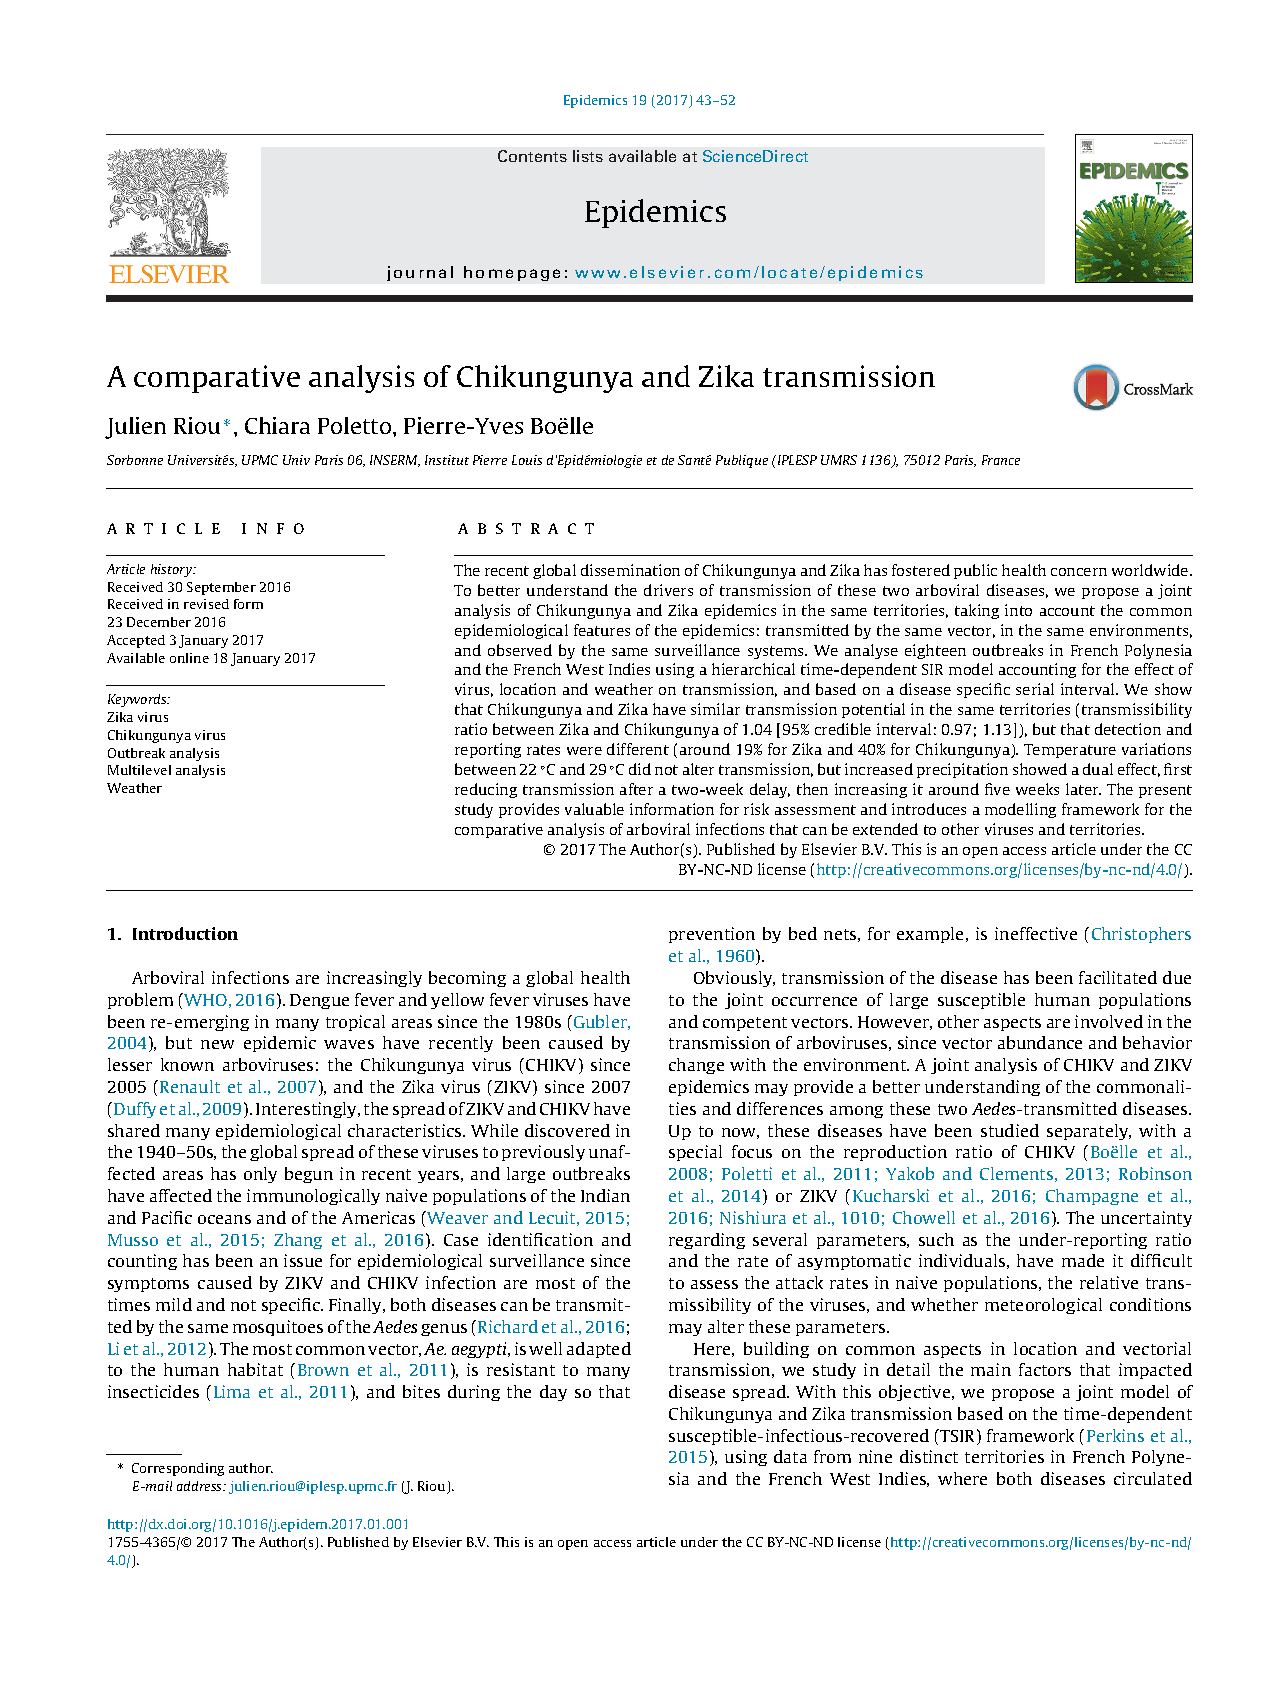
\includepdf[pages={1-10}]{Articles/epidemics.pdf}
\cleardoublepage

\section{Principaux résultats}

Le modèle hiérarchique utilisé dans cette étude, intégrant les effets respectifs du virus, du territoire et des conditions météorologiques, permet d'obtenir une bonne description des dynamiques épidémiques observées lors de la circulation du chikungunya et du Zika en Polynésie française et aux Antilles françaises.
Les résultats répondent aux objectifs fixés :
\begin{itemize}
\item[(1)] Lorsque deux épidémies de chikungunya et de Zika surviennent successivement dans territoire \guillemotleft typique\guillemotright\ des régions étudiées, on s'attend à retrouver des niveaux de transmissibilité équivalents ($\beta_D=1,04$ ; intervalle de crédibilité à 95\% 0,97-1,13) mais un taux de signalement plus faible pour le Zika ($\omega=0,37$ ; IC95\% 0,34-0,40).
Cela correspond à des estimations de $\mathcal{R}_0$ moyennes toutes îles confondues de 1,82 (IC95\% 1,52-2,17) pour le chikungunya et de 1,87 (IC95\% 1,55-2,24) pour le Zika, un peu plus basses mais comparables à d'autres études sur le chikungunya ou le Zika dans les mêmes territoires \cite{kucharski2016transmission,Champagne064949,cauchemez2014local,nishiura2016transmission}, même si les différences d'approche méthodologique rendent la comparaison directe difficile.
Les estimations du taux de signalement sont de 41\% (IC95\% 29-55) pour le chikungunya et de 19\% (IC95\% 12-29) pour le Zika, ce qui est cohérent avec les différences connues entre les deux maladies concernant la proportion de cas symptomatiques (estimée à environ 30\% pour le Zika contre 80\% pour le chikungunya). 
D'autre part, cela suggère que les différences entre virus pouvant avoir une influence sur la transmissibilité, comme par exemple la probabilité de transmission par piqûre, n'ont que peu d'effet comparativement à d'autres facteurs liés aux vecteurs et aux hôtes.
\vspace{.3em}
\item[(2)] La température locale moyenne dans les huit semaines précédentes ne semble pas avoir influencé les niveaux de transmission durant les épidémies. Toutefois, la température est restée globalement stable durant ces épidémies, presque constamment entre 25 et 28$^{\circ}$C, et seulement un peu plus faible aux îles Australes, ce qui pourrait expliquer l'absence d'effet détecté contrairement à d'autres études \cite{li_rainfall_1985,barrera_population_2011,lu_time_2009}. Au contraire, on retrouve un effet sensible des précipitations sur la transmission : après la pluie, les niveaux de transmission diminuent d'environ 20\% pendant une à deux semaines ($\beta_{T,2}=0,81$ ; IC95\% 0,66-0,98), puis sont accrus après un délai de quatre à six semaines d'environ 30\% ($\beta_{T,5}=1,30$ ; IC95\% 1,09-1,56). Ce délai de quatre à six semaines est intéressant car il correspond au temps de développement des moustiques du stade larvaire au stade adulte \cite{barrera_population_2011}, ce qui fournit une interprétation plausible de ce résultat.
\vspace{.3em}
\item[(3)] L'estimation des paramètres de variance inter-île montrent une hétérogénéité résiduelle marquée de la transmissibilité et du taux de signalement. 
D'autres études ont aussi retrouvé des différences entre territoires \cite{kucharski2016transmission,Champagne064949,cauchemez2014local,nishiura2016transmission,chowell_using_2016,funk2016comparative}. 
Le modèle permet d'attribuer cette hétérogénéité aux caractéristiques spécifiques des îles, mais il est difficile d'aller au delà avec les données disponibles.
On observe une plus faible transmissibilité aux Antilles qu'en Polynésie, ce qui pourrait s'expliquer par des différences de population, d'environnement ou encore d'abondance et de composition des populations de vecteurs.
En particulier, le vecteur {\em Ae. polynesiensis}, présent seulement en Polynésie, a été considéré comme un vecteur possible de chikungunya et de Zika \cite{richard2016vector}.
Concernant le taux de signalement, il est probable que l'hétérogénéité soit liée à des différences d'organisation du système de soin et de surveillance. 
On observe d'ailleurs une tendance à des taux de signalement plus élevés dans les îles les moins peuplées, comme les îles Australes, les îles Marquises ou Saint-Martin.
Les taux de signalement sont aussi plus faibles en Martinique, sans qu'il existe d'explication évidente.
Des données plus précises, par exemple de type longitudinales, permettraient d'aller plus loin dans l'explication de ces différences et d'estimer l'influence de certains aspects comme par exemple la mobilité humaine \cite{stoddard2013house}, la qualité des habitations \cite{reiter_texas_2003}, ou encore le mode de gestion de l'eau et des ordures \cite{monath1994dengue}.

\end{itemize}

\section{Commentaires et perspectives}

Dans ce travail, nous avons développé un modèle hiérarchique innovant permettant l'analyse conjointe d'épidémies successives de chikungunya et de Zika dans neuf zones, quantifiant les effets respectifs du virus, des conditions météorologiques et du territoire sur les dynamiques de transmission et de surveillance.
Cela a permis de montrer les niveaux de transmission observés de ces épidémies dépendent peu du virus en cause, mais sont influencés par les conditions météorologiques, en particulier les précipitations.
Une large part de la variabilité entre les îles est liée à des caractéristiques locales, non-observées ici.
D'autres études utilisant des données plus détaillées pourraient permettre de mieux comprendre quelles sont les caractéristiques locales les plus influentes, ce qui pourrait mener à l'identification de nouvelles cibles d'action pour la prévention et le contrôle de ces maladies.
Ces résultats reposent toutefois sur plusieurs hypothèses limitantes, en particulier une part d'incertitude dans la construction mécaniste de l'intervalle de génération.

Pour autant, cette étude fournit des informations importantes.
Le fait que des épidémies successives de chikungunya et de Zika aient des niveaux de transmissibilité équivalents, mais des taux de signalement différents en lien avec la proportion de cas symptomatiques spécifique à chaque maladie est un résultat attendu, qu'il fallait pourtant démontrer et quantifier.
Des conclusions assez proches ont d'ailleurs été retrouvées dans une comparaison des épidémies de Zika et de dengue sur l'île de Yap \cite{funk2016comparative}.
De façon générale, les études d'épidémiologie comparée restent rares.
Par exemple, un travail a indiqué un coefficient de corrélation de 0,62 entre les nombres de reproductions de vagues successives de grippe aux \'Etats-Unis d'Amérique en 1889 et 1918 \cite{valleron2010transmissibility}.
Pourtant, l'extension de ce type de travail permet d'améliorer la compréhension des liens entre épidémies, et donc de certaines caractéristiques générales.
Cela pourrait avoir un effet bénéfique sur la préparation de la communauté internationale en cas de nouvelle émergence, en particulier de maladies transmises par les moustiques du genre {\em Aedes}.